\begin{frame}
    \begin{figure}
        \hspace*{-320pt}
\includegraphics[width=1.0cm]{vstu-logo}
    \end{figure}
    \vspace{2em}
    \begin{center}
        \large
        \textbf{Метод кластеризации предпочтений жителей города по перемещению}\\
    \end{center}
    \vspace{2em}
    \begin{flushleft}
        \hspace{12em}Автор:~Чечеткин~И.~А.\\
        \hspace{12em}группа:~САПР-2п1\\
        \hspace{12em}Руководитель:~Щербаков~М.~В.
    \end{flushleft}
    \vspace{3em}
    \centeringВолгоград \the\year\ г.
\end{frame}

\begin{frame}
    \frametitle{Цели и задачи}
    \textbf{Целью} данной работы являлась разработка метода кластеризации предпочтений жителей, выраженных в паре геораспределенных объектов <<отправление-назначение>>, с учетом городского рельефа.

    В данной работе рассматриваются к решению следующие задачи:
    \begin{itemize}
        \item генерация псевдореалистичных данных о перемещениях жителей;
        \item разработка метрики расстояний, учитывающей рельеф местности;
        \item модификация и использование существующих алгоритмов для кластеризации геораспределенных данных с разработанной метрикой расстояний;
        \item представление построенных кластеров на карте.
    \end{itemize}
\end{frame}

\begin{frame}
    \frametitle{Актуальность}
    Изменения в городской среде требуют формирования новых механизмов планирования инфраструктуры города. 
    Для получения эффективных результатов, следует осуществлять принятие решений на основе актуальных 
    данных, отражающих предпочтения жителей.
    \begin{figure}
        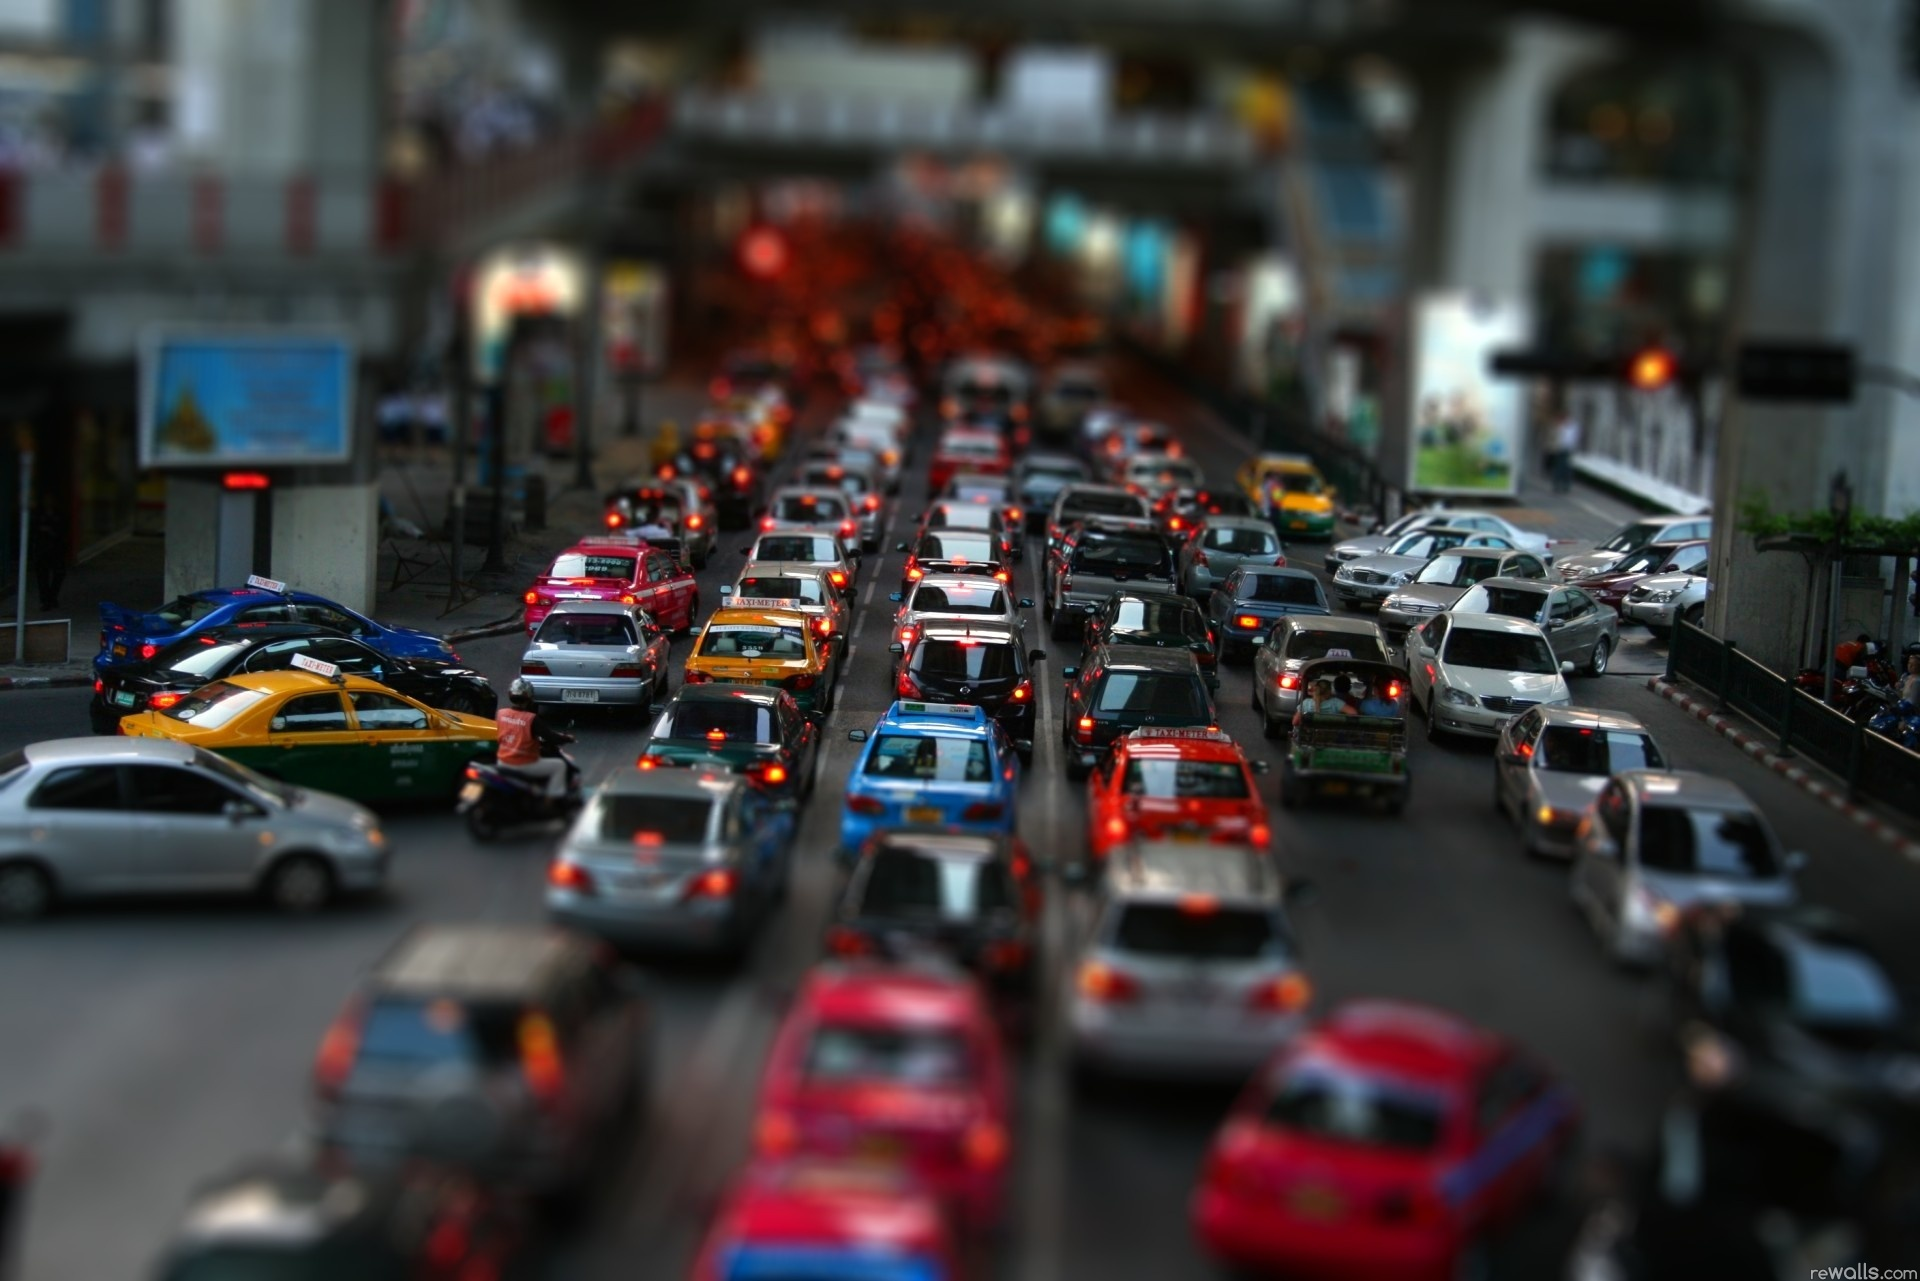
\includegraphics[width=0.7\textwidth]{traffic-jam}
    \end{figure}
\end{frame}

\begin{frame}
    \frametitle{Научная новизна}
    Научная новизна работы обусловлена:
    \begin{itemize}
        \item предложена автоматизация процесса построения сети остановочных пунктов без участия транспортного инженера;
        \item предложен метод, основанный на использовании данных о предпочтении жителей для построения сети остановочных пунктов;
        \item разработан метод кластеризации географических точек с учетом препятствий.
    \end{itemize}
\end{frame}

\begin{frame}
    \frametitle{Анализ предметной области}
    Существующие инструменты для проведения комплексного анализа:
    \begin{itemize}
        \item WEKA;
        \item RapidMiner;
        \item R;
        \item MatLab;
        \item Scikit-Learn.
    \end{itemize}
    \begin{figure}
        \centering
        
\includegraphics[height=1.5cm]{weka-logo}\quad
        
\includegraphics[height=1.5cm]{rapidminer-logo}\\
        
\includegraphics[height=1.1cm]{R-logo}\quad
        
\includegraphics[height=1.1cm]{matlab-logo}\quad
        
\includegraphics[height=1.1cm]{sklearn-logo}
    \end{figure}
\end{frame}

\begin{frame}
    \frametitle{Постановка задачи}
    \textbf{Объект исследования} -- кластеризация предпочтений жителей города по перемещению, выраженных в виде пары точек <<Пункт отправления~-- пункт назначения>>, каждая из которых содержит две координаты~-- широту и долготу.\\\vspace{1em}

    \textbf{Предмет исследования} -- разработка и применение методов кластеризации предпочтений жителей, учитывающих элементы рельефа местности.\\\vspace{1em}

    \textbf{Гипотеза исследования} -- Использование данных о перемещениях жителей и автоматизация построения сети остановочных пунктов и маршрутной сети позволяют построить оптимальную сеть маршрутов общественного транспорта.
\end{frame}

\begin{frame}
    \frametitle{Входные данные}
    \begin{figure}
        \centering
        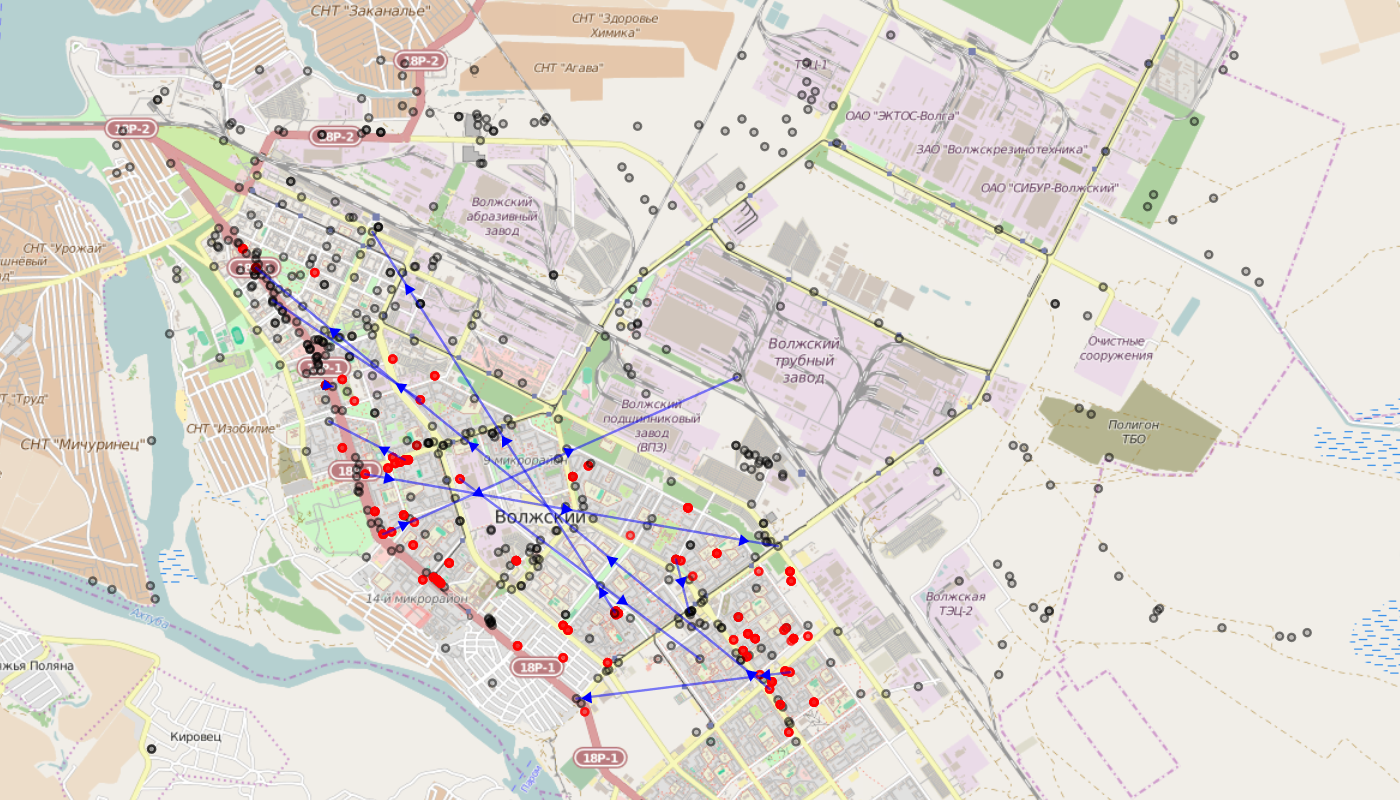
\includegraphics[width=\textwidth]{points-01}
    \end{figure}
\end{frame}

\begin{frame}
    \frametitle{Входные данные}
    \begin{figure}
        \centering
        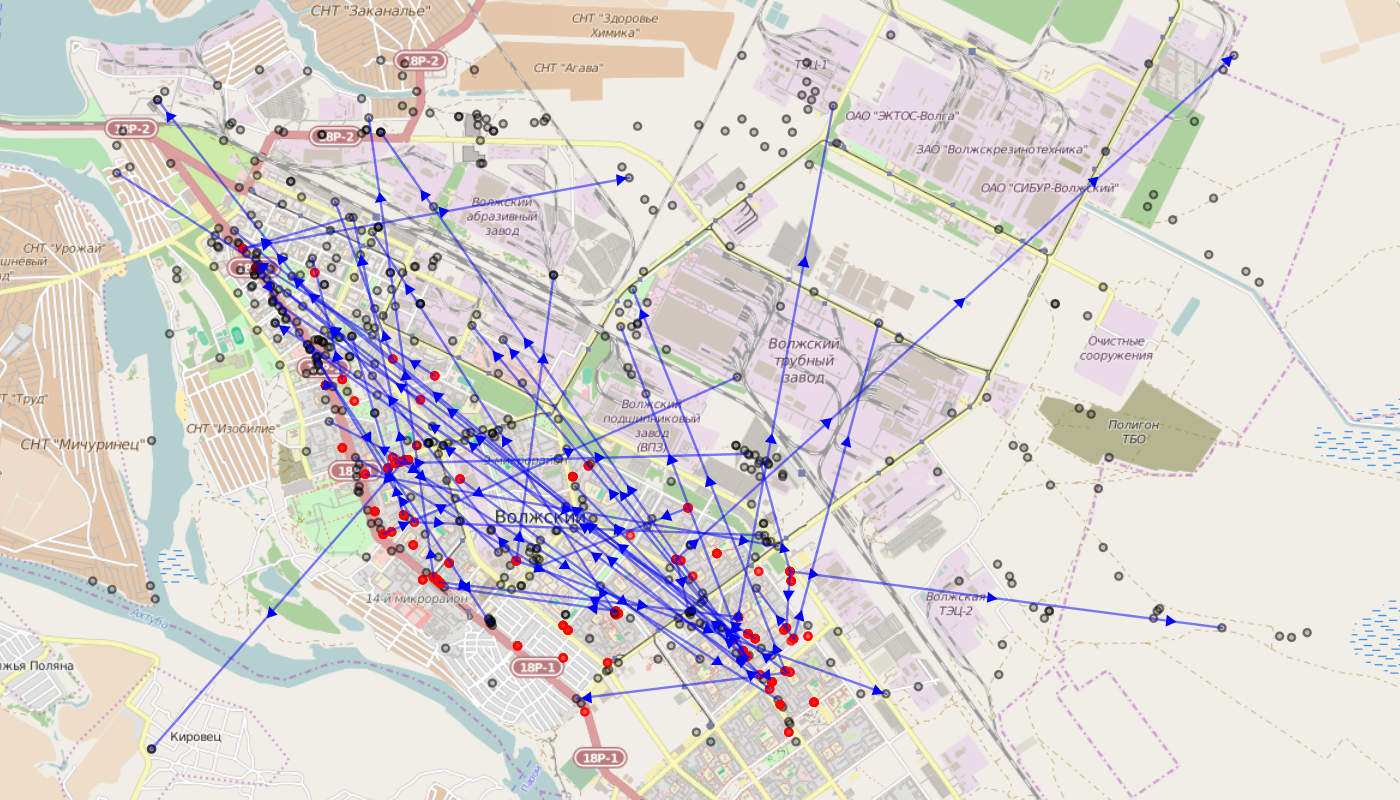
\includegraphics[width=\textwidth]{points-02}
    \end{figure}
\end{frame}

\begin{frame}
    \frametitle{Входные данные}
    \begin{figure}
        \centering
        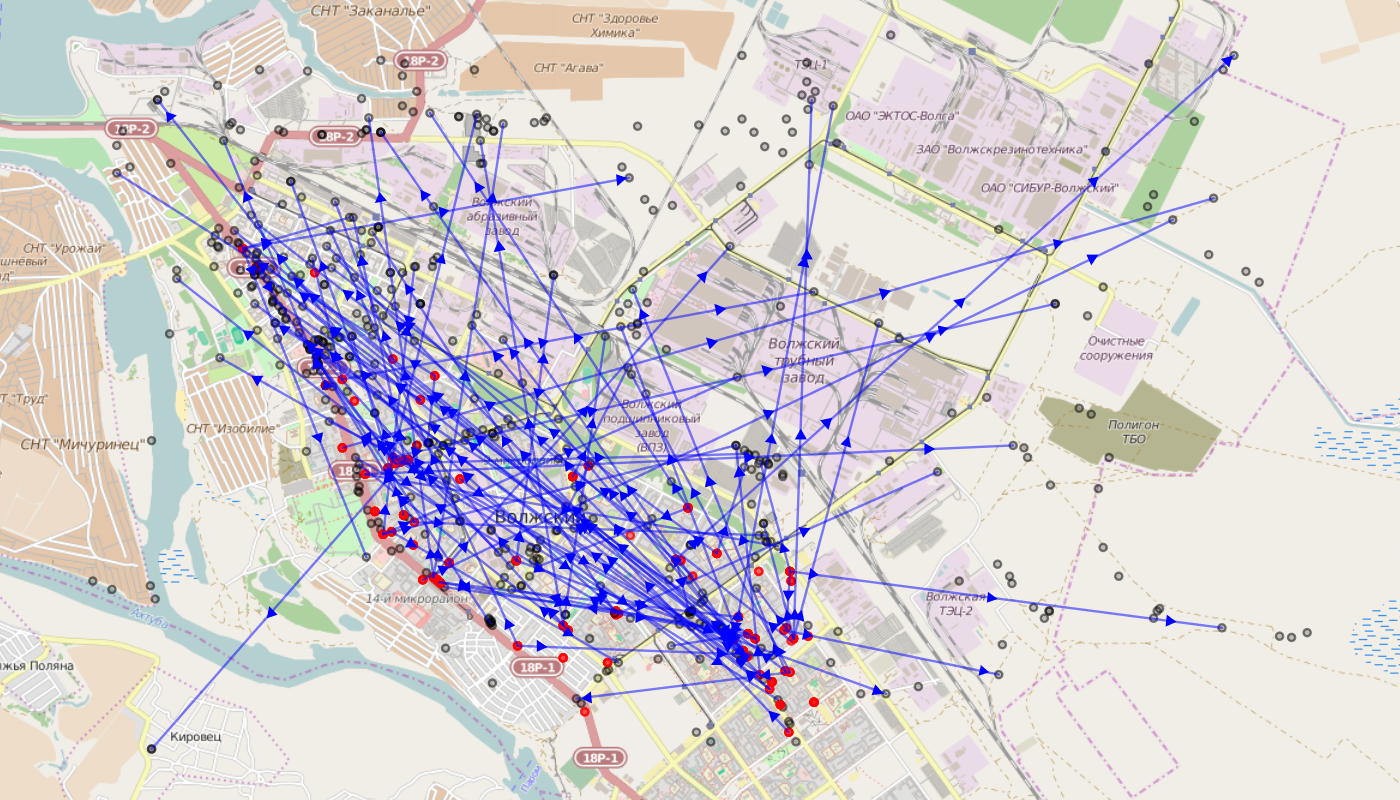
\includegraphics[width=\textwidth]{points-03}
    \end{figure}
\end{frame}

\begin{frame}
    \frametitle{Входные данные}
    \begin{figure}
        \centering
        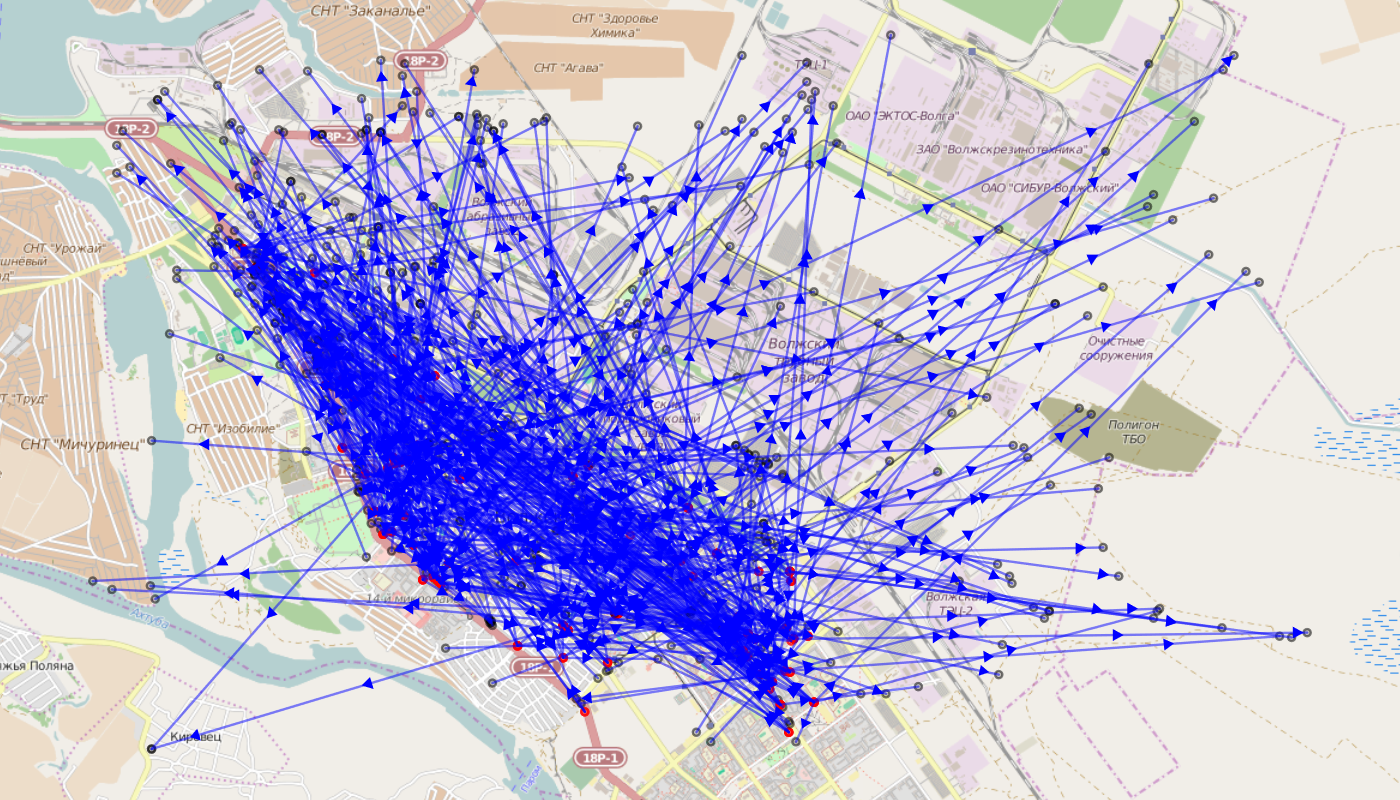
\includegraphics[width=\textwidth]{points-04}
    \end{figure}
\end{frame}

\begin{frame}
    \frametitle{Входные данные}
    \framesubtitle{Сгенерированные данные}
    \begin{figure}
        \centering
        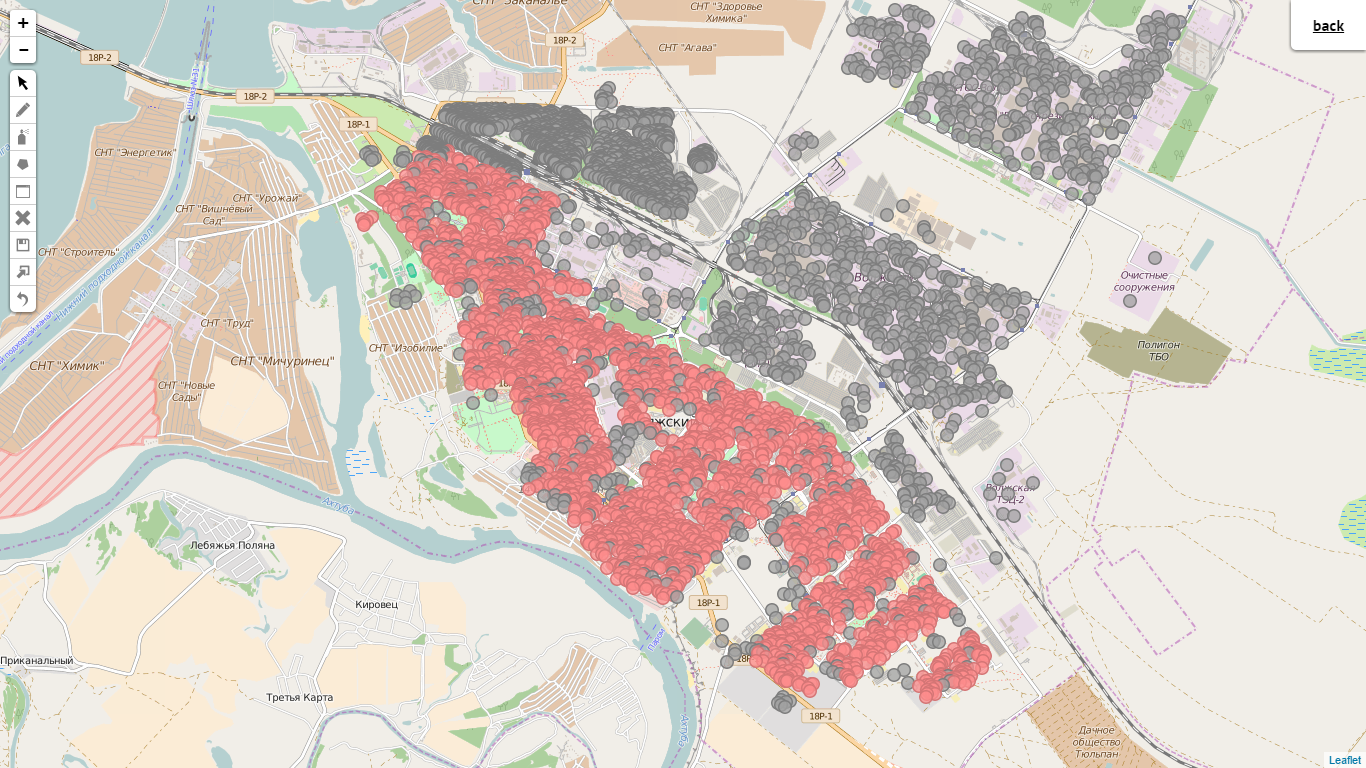
\includegraphics[width=\textwidth]{full}
    \end{figure}
\end{frame}

\begin{frame}
    \frametitle{Метрика}
    \begin{figure}
        \centering
        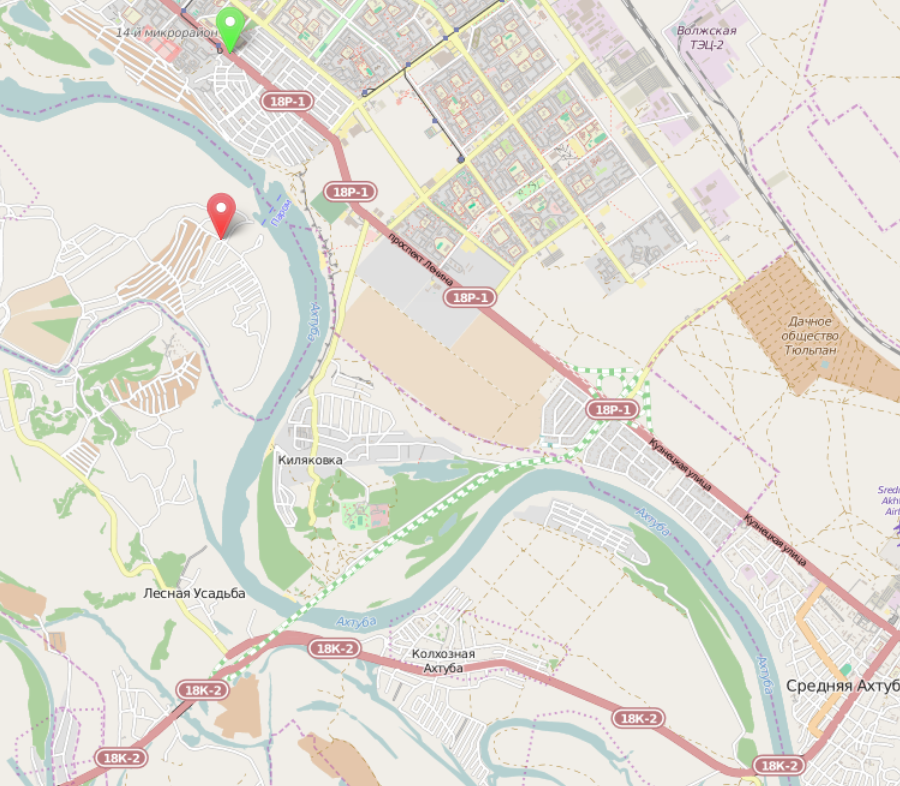
\includegraphics[height=5.2cm]{2p_riv_1}\ \
        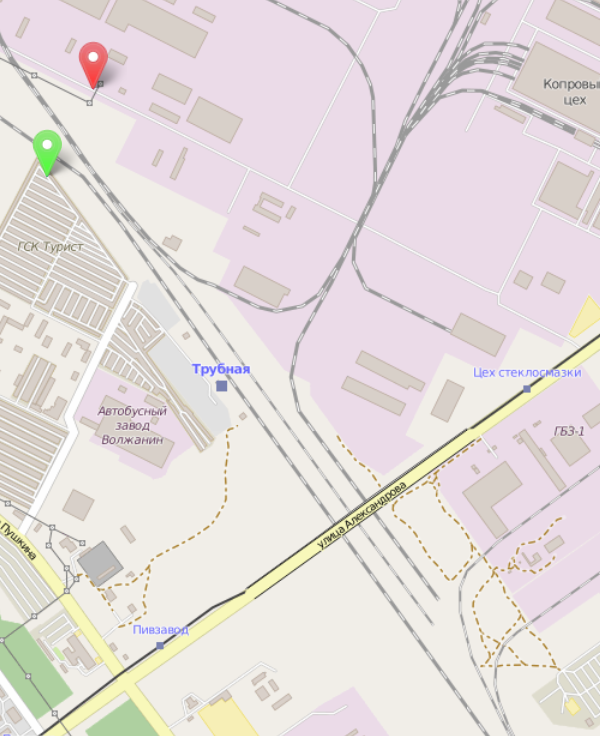
\includegraphics[height=5.2cm]{2p_rail_1}
    \end{figure}
\end{frame}

\begin{frame}
    \frametitle{Метрика}
    \begin{figure}
        \centering
        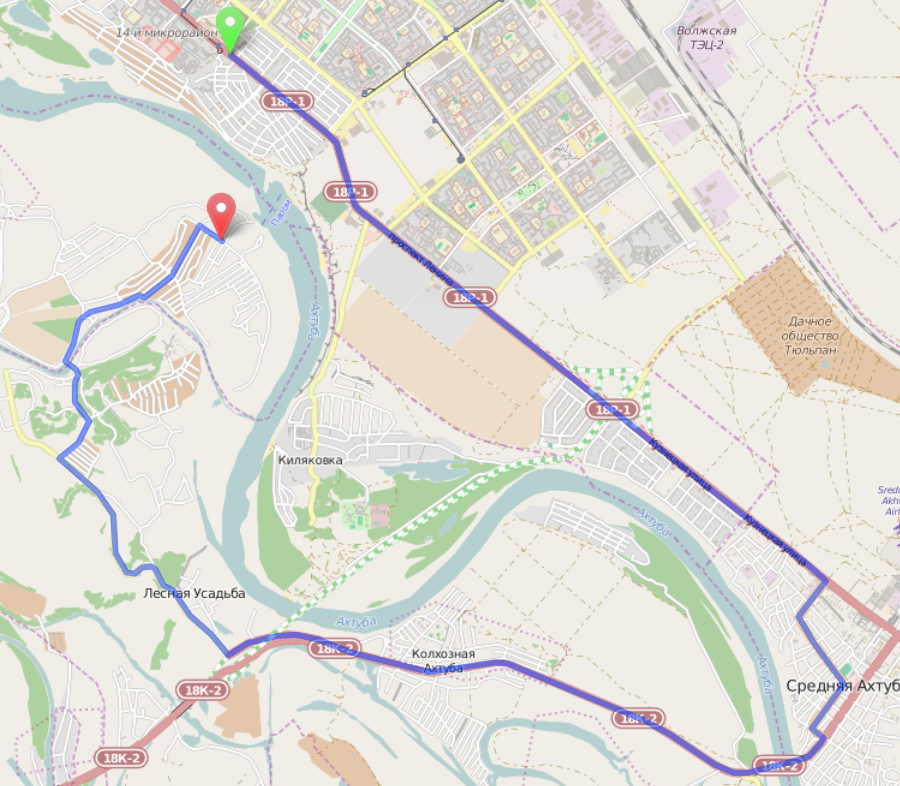
\includegraphics[height=5.2cm]{2p_riv_2}\ \
        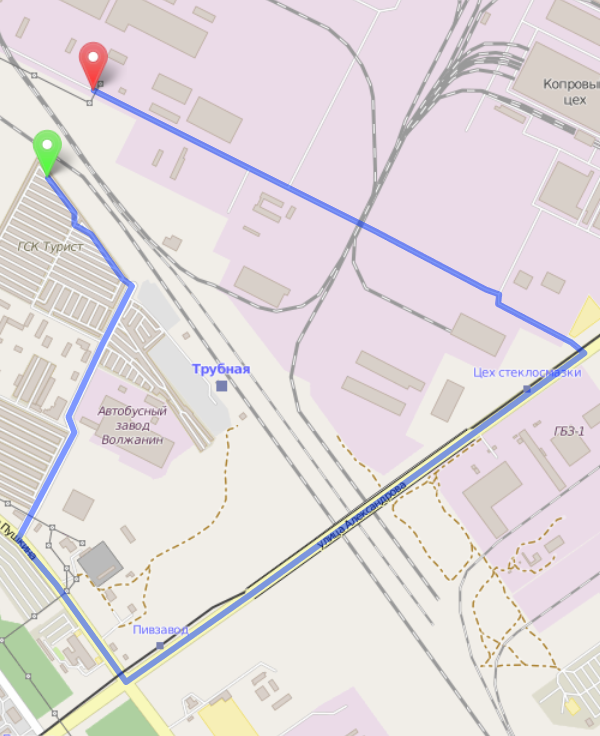
\includegraphics[height=5.2cm]{2p_rail_2}
    \end{figure}
\end{frame}

\begin{frame}
    \frametitle{Метрика}
    \framesubtitle{Пример работы OSRM}
    \begin{figure}
        \centering
        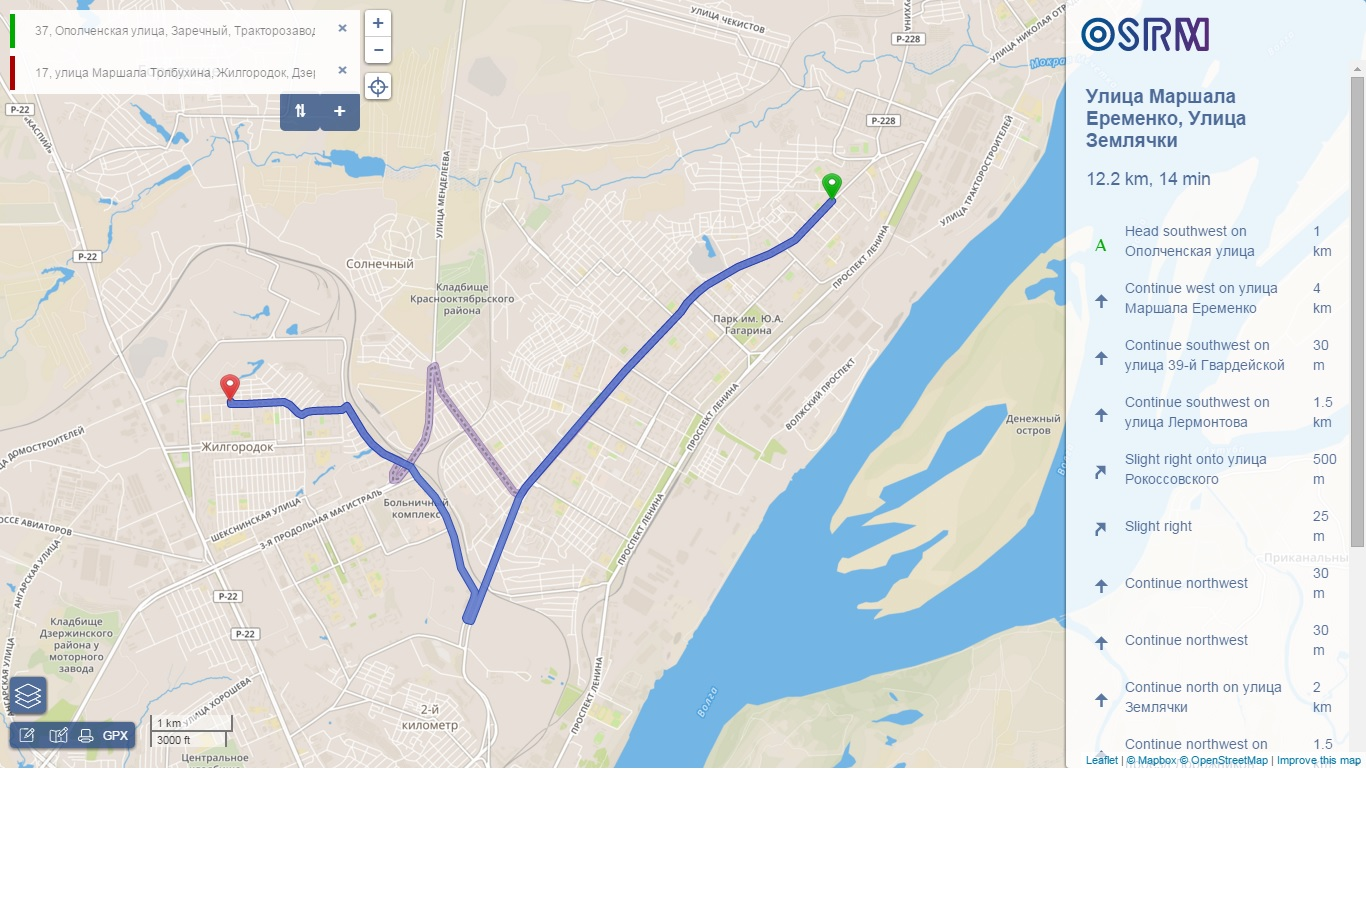
\includegraphics[width=\textwidth]{osrm}
    \end{figure}
\end{frame}

\begin{frame}
    \frametitle{Алгоритмы кластеризации}
    \begin{figure}
        \centering
        \vspace*{-1em}
        \hspace*{-2em}
        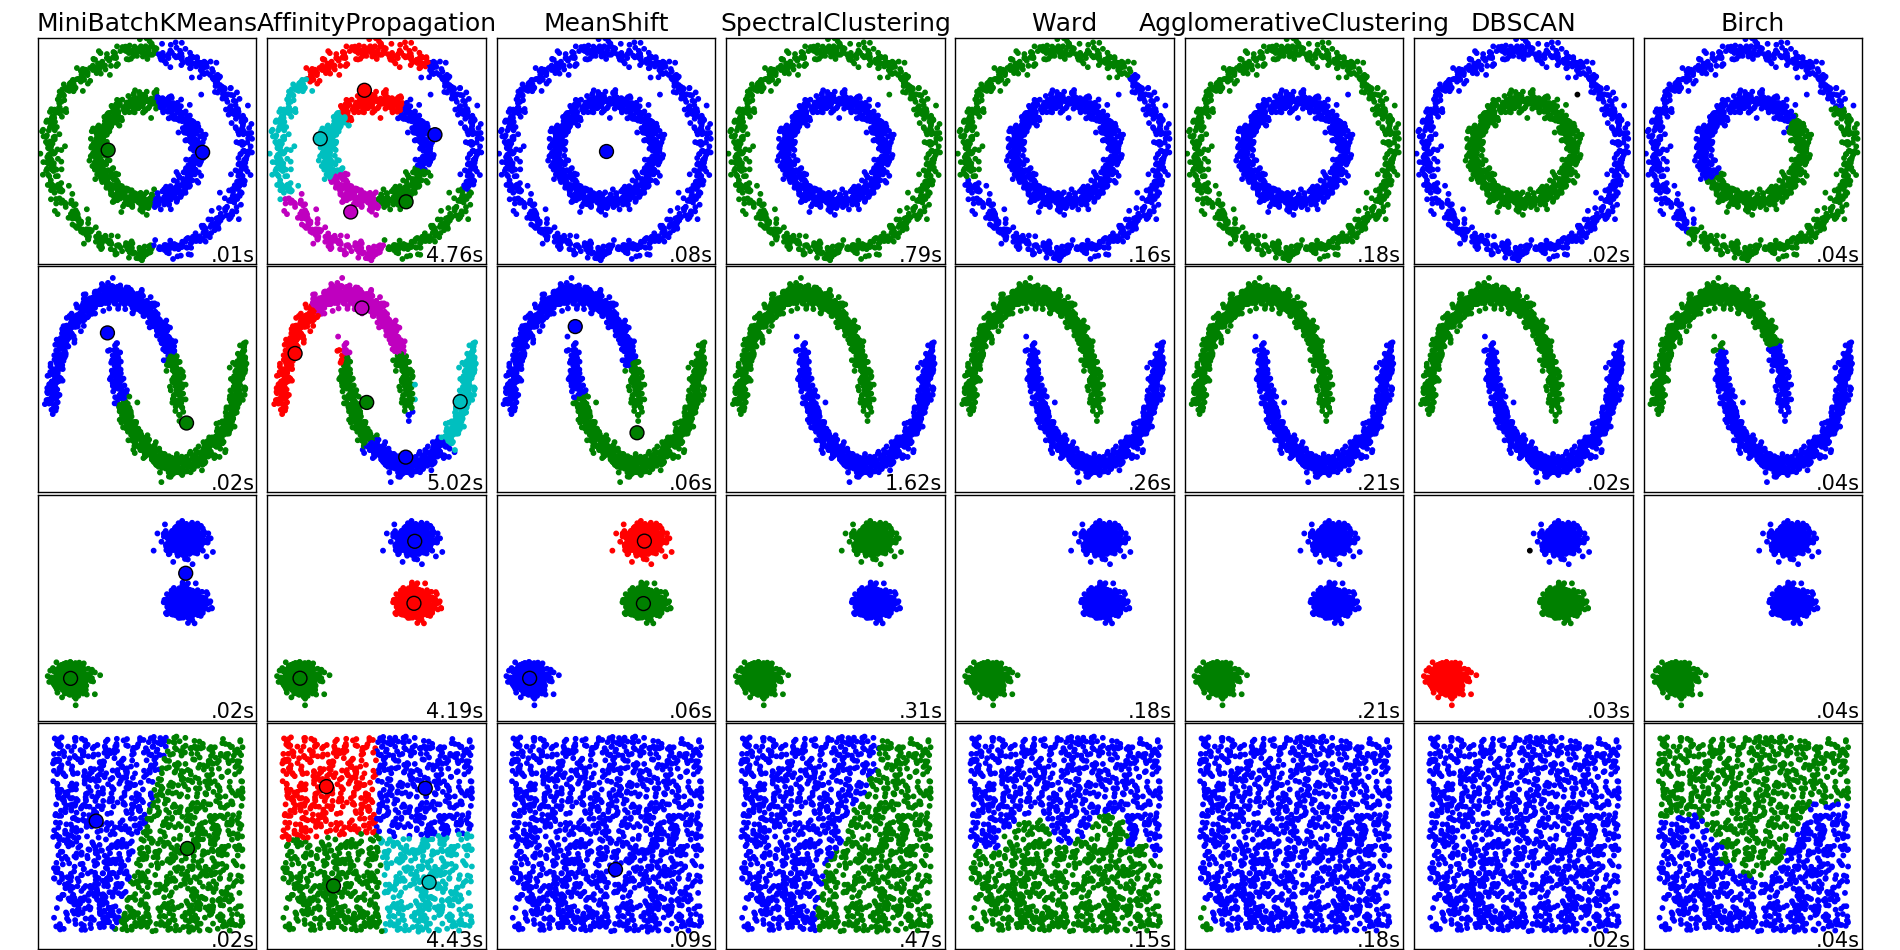
\includegraphics[width=1.15\textwidth]{scikit-clustering}
    \end{figure}
\end{frame}

%\begin{frame}
%    \frametitle{Алгоритмы кластеризации}
%    \framesubtitle{Алгоритм k-means}
%    \begin{figure}[h!]
%        \centering
%        \raisebox{-1.5ex}{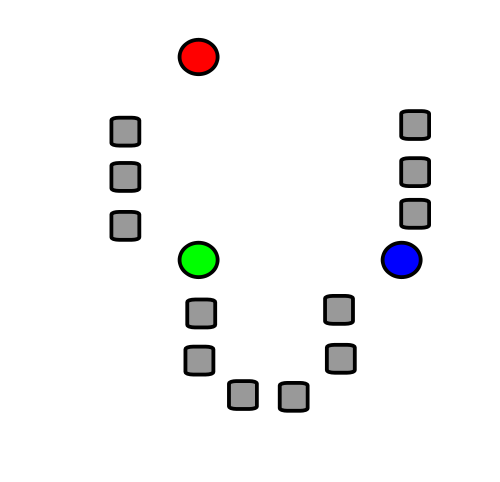
\includegraphics[width=.245\textwidth]{km_step1}}
%        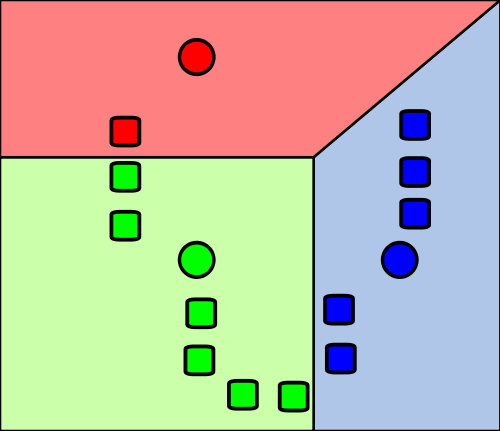
\includegraphics[width=.245\textwidth]{km_step2}
%        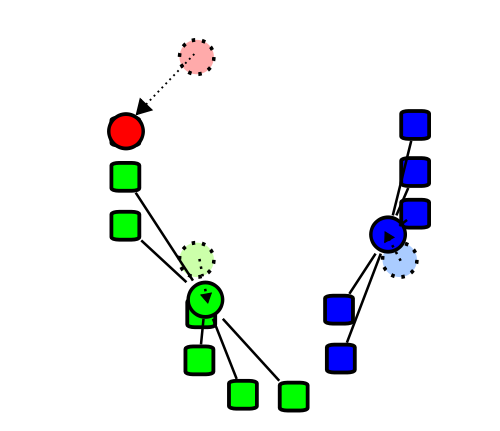
\includegraphics[width=.245\textwidth]{km_step3}
%        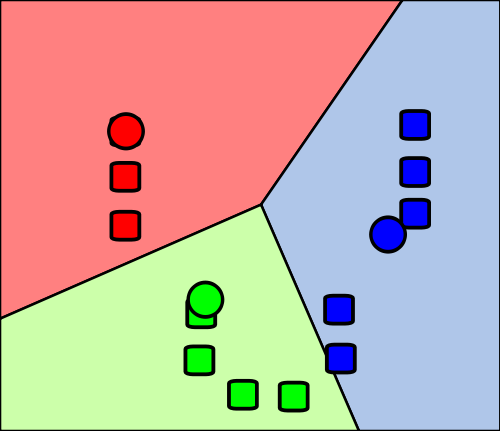
\includegraphics[width=.245\textwidth]{km_step4}
%    \end{figure}
%\end{frame}

\begin{frame}
    \frametitle{Алгоритмы кластеризации}
    \framesubtitle{Алгоритм k-means}
    \begin{figure}
    \scriptsize
    \begin{algorithm}[H]
        \KwData{\( X \), \( k \), \( C_0 \), \( I \).}
        \KwResult{\( C \), \( L \).}
        1. \( C = C_0 \), \( L_0 = \varnothing \), \( i = 0\)\;
        2. \While{\( L != L_0\) и \( i < I \)}{
            1. \( L_0 = L \), \( A = \varnothing \), \( \mu = \varnothing \)\;
            2. \ForEach{\( x \in X \)}{
                1. \( r = \varnothing \)\;
                2. \ForEach{\( c \in C \)}{
                    1. Рассчитать \( r_{xc} = \rho(x, c) \)\;
                    2. \( r = r + \{ r_{xc} \} \)\;
                }
                3. \( L[x] = C[\min(r)] \)\;
                4. \( A[C[\min(r)]] = A[C[\min(r)]] + \{x\}\)\;
            }
            3. \ForEach{\( c \in C \)}{
                1. \( \mu[c] = \sum(A[c])\,/ \abs{A[c]} \)\;
                2. \( c = \mu[c] \)\;
            }
            4. \( i = i + 1 \)\;
        }
    \end{algorithm}
    \vspace*{-1.5em}
    \end{figure}
\end{frame}

\begin{frame}
    \frametitle{Проектирование программного продукта}
    \small
    Используемые технологии:
    \begin{itemize}
        \item Python 3 (\url{https://www.python.org/})
        \item OSRM (\url{http://project-osrm.org/})
        \item OpenStreetMap (\url{https://www.openstreetmap.org})
        \item Leaflet (\url{http://leafletjs.com/})
    \end{itemize}
    Исходный код доступен по следующей ссылке:\\
    {\footnotesize\url{https://github.com/vstu-cad-stuff/clustering/tree/master}}\\\vspace{1em}
    Результаты работы реализованных алгоритмов:\\
    \url{https://vstu-cad-stuff.github.io/clustering/}
\end{frame}

\begin{frame}
    \frametitle{Результат}
    \framesubtitle{Евклидова метрика в проекции Меркатора}
    \begin{figure}[ht!]
        \centering
        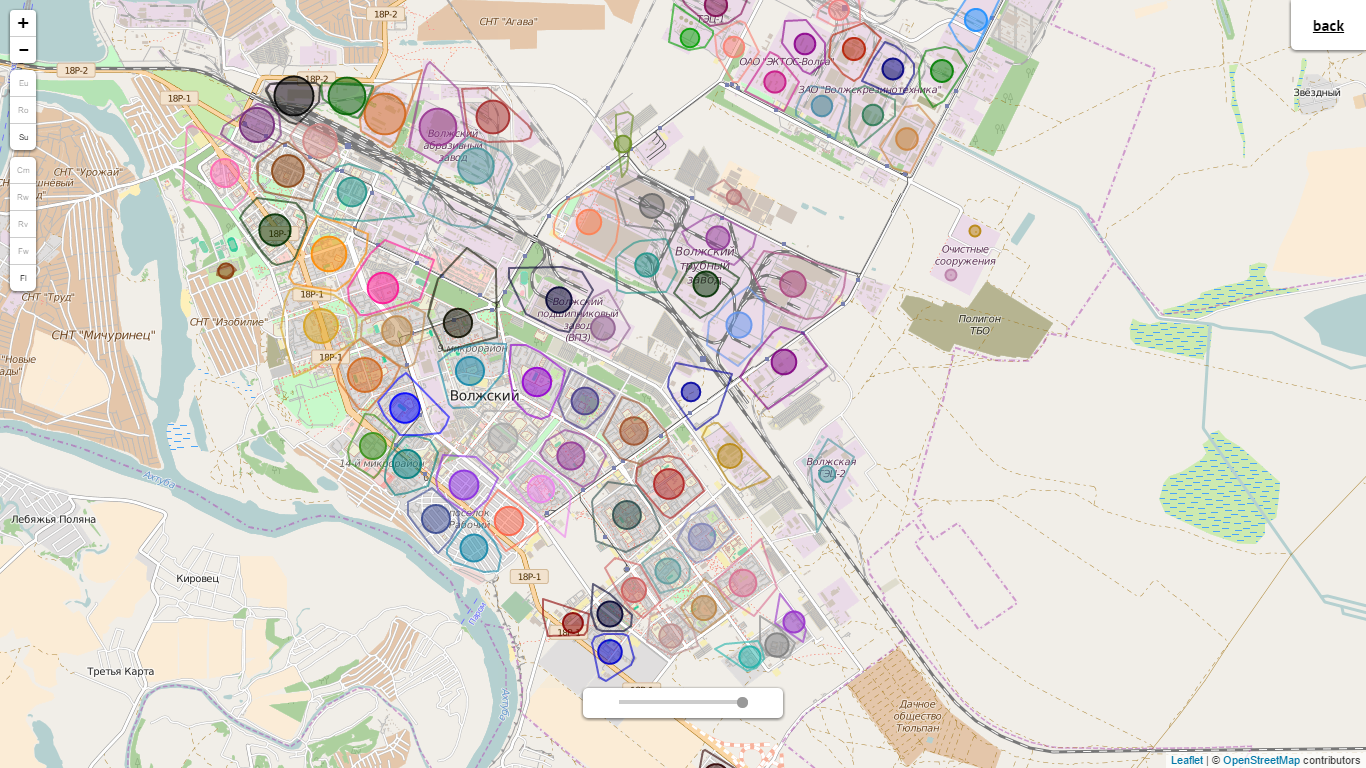
\includegraphics[width=\textwidth]{full_surface}
    \end{figure}
\end{frame}

\begin{frame}
    \frametitle{Результат}
    \framesubtitle{Построение по дорожной сети}
    \begin{figure}[ht!]
        \centering
        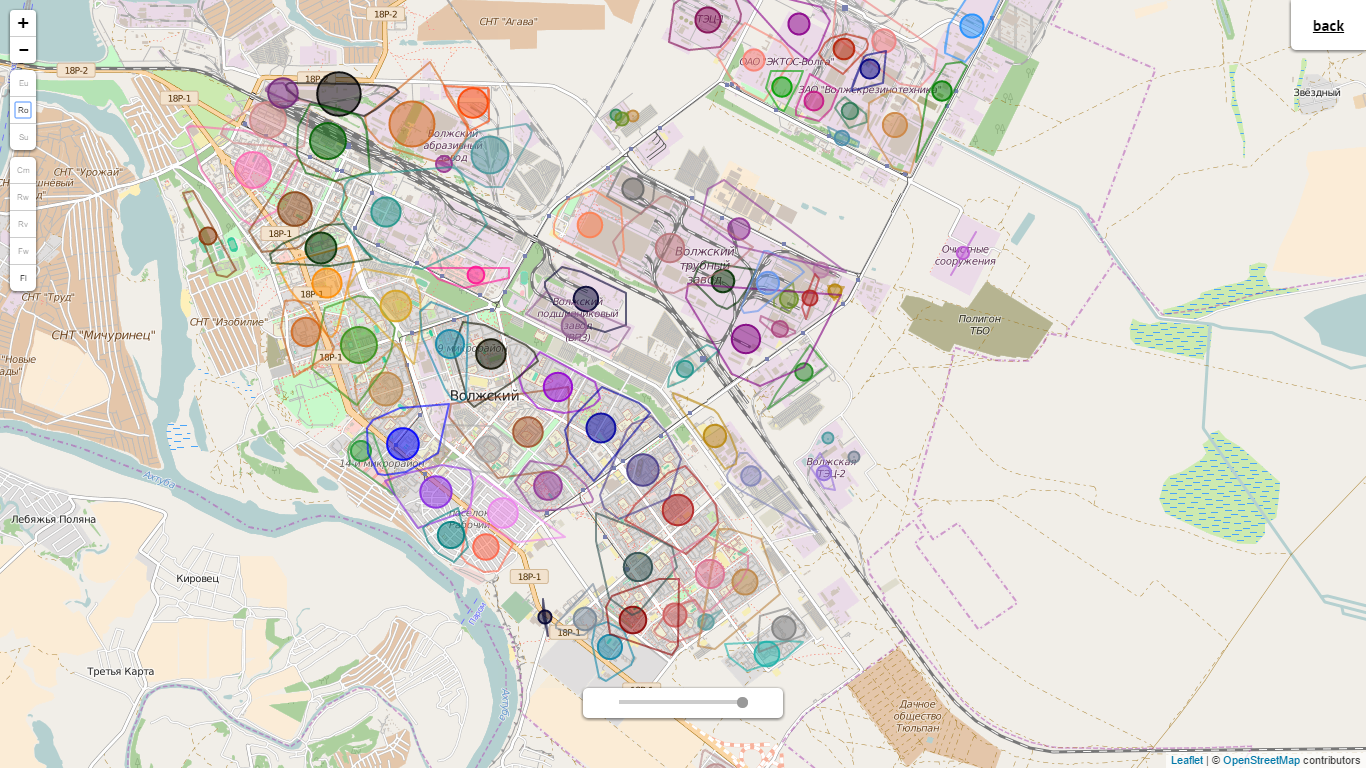
\includegraphics[width=\textwidth]{full_route}
        \vspace*{-1ex}
    \end{figure}
    {\small\url{http://vstu-cad-stuff.github.io/clustering/kmeans/}}
\end{frame}

\begin{frame}
    \frametitle{Результат}
    \framesubtitle{Сдвиг центров кластеров к участкам дорожной сети}
    \begin{figure}[ht!]
        \centering
        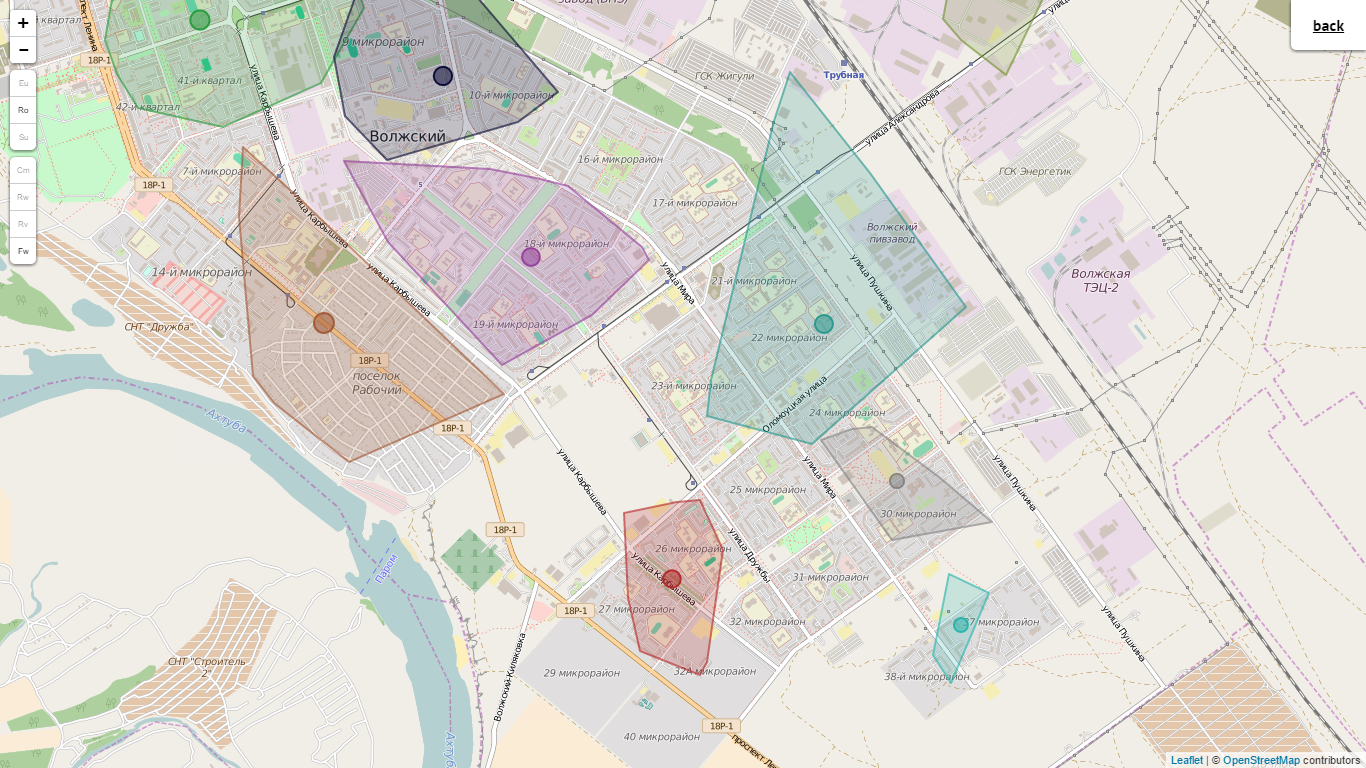
\includegraphics[width=\textwidth]{terminals-more}
        \vspace*{-1ex}
    \end{figure}
    {\small\url{http://vstu-cad-stuff.github.io/clustering/terminals/}}
\end{frame}

\begin{frame}
    \frametitle{Основные результаты работы}
    В ходе проведения научной работы были получены следующие результаты:
    \begin{itemize}
        \item предложен алгоритм формирования сети остановочных пунктов на основе кластеризации данных о предпочтениях жителей;
        \item изучены алгоритмы, используемые для кластеризации распределенных данных;
        \item реализована метрика расстояний, основанная на расчете расстояния по графу дорог;
        \item реализован алгоритм формирования сети остановочных пунктов на основе кластеризации данных о предпочтениях жителей;
        \item проверена эффективность реализованного алгоритма на сгенерированных наборах данных.
    \end{itemize}
\end{frame}

\begin{frame}
    \frametitle{Публикации}
    \scriptsize
    \begin{thebibliography}{10}
        \bibitem{first} Strategway: web solutions for building public transportation routes using big geodata 
            analysis / Golubev A., Chechetkin I., Solnushkin K.S., Sadovnikova N., Parygin D., Shcherbakov M., 
            Brebels A. // Proceedings of The 17th International Conference on Information Integration and 
            Web-based Applications \& Services (iiWAS2015) (December 11 - 13, 2015 Brussels, Belgium) 
            ACM New York, New York pp. 665 - 668
        \bibitem{second} Комплекс инструментов интеллектуального анализа данных strategway для поддержки 
            принятия решений по управлению развитием инфраструктуры города / Садовникова Н.П., Щербаков М.В., 
            Парыгин Д.С., Солнушкин К.С., Голубев А.В., Чечеткин И.А. // В сборнике: Развитие средних 
            городов: замысел, модели, практика Материалы III Международной научно-практической конференции. 
            Волгоград, 2015. С. 147-150
        \bibitem{third} Автоматизация поддержки принятия решений по разработке маршрутов общественного 
            транспорта на основе анализа данных о корреспонденциях жителей / М. В. Щербаков, 
            Н. П. Садовникова, Д. С. Парыгин, А. В. Голубев, И. А. Чечеткин // Вестник компьютерных и 
            информационных технологий. -- М. : Издательский дом <<Спектр>>, 2016. -- В печати.
    \end{thebibliography}
\end{frame}

\begin{frame}
    \frametitle{Вопросы}
    \begin{minipage}{0.3\textwidth}
        \begin{figure}[ht!]
            \centering
            
\includegraphics[width=\textwidth]{questions}
        \end{figure}
    \end{minipage}
    \begin{minipage}{0.6\textwidth}
        \begin{center}
            Чечеткин Илья Александрович, САПР-2п1,
            \href{mailto:illaech@gmail.com}{illaech@gmail.com}
        \end{center}
    \end{minipage}
\end{frame}
